\ustcsetup{
  cite-style = authoryear,
}

% \chapter{背景噪声干涉在DAS成像中的应用}
\chapter{基于DAS观测的背景噪声成像:以2020年白家疃实验为例}

在本章,我们先系统回顾背景噪声干涉的原理及其证明,讨论不同背景噪声场的假设下,噪声干涉理论证明结果的一致性。
然后介绍我们基于SeisNoise.jl~\citep{clements2021seisnoise},利用Julia语言的并行计算,设计了大规模背景噪声互相关运算的框架。
在介绍利用DAS进行背景噪声成像之前,我们先简要介绍DAS传感的原理与应用,然后介绍2020背景白家疃DAS观测实验及其背景噪声成像工作。

\section{背景噪声干涉理论}

\subsection{多模态叠加}
多模态叠加(Normal-mode summation)理论最初在研究地球自由震荡中被提出,在此我们将其应用于有限体内的声学介质中。
声学中的控制方程,即声波方程表示如下:
\begin{align}
    \frac{1}{\kappa (x)} \frac{\partial^2}{\partial t^2} u(x,t) 
    - 
    \frac{\partial}{\partial x_i} \bigl( \frac{1}{\rho(x)} \frac{1}{\partial x_i }  u(x,t)     \bigl)
    =
    f(x,t)
    \label{equ:ac-wave}
\end{align}
其中$x$是位置向量,$\kappa$是体积弹性模量(bulk modulus),$\rho$是密度,$f$是激发声波波场的外力。
当我们忽略$f$的存在,上述方程的多模态解可以表示为:
\begin{align}
    u_p(x,t) = s_p(x) cos(\omega_p t + \varPhi_p)
    \label{equ:ac-nm}
\end{align}
其中$s_p(x)$是空间模态形状(spatial mode shape)或者称为特征函数(eigenfunction),$\omega_p$是模态的频率,$\varPhi_p$是模态的相位。
对于空间正交性,我们有$\int s_m(x)s_n(x)dx = 0, m\neq n$;
针对时间正交性,我们有$\int cos(\omega_m t + \varPhi_m ) cos(\omega_n t + \varPhi_n ) dt = 0, \omega_m \neq  \omega_n   $
在这里我们假设不同模态拥有的频率不一样。

对于任意一个模态,因为空间正交性,格林函数可以写成\citep{snieder2015guided}:
\begin{align}
    G_p(x,x_s,t)=
    \begin{cases}
        \frac{s_p(x)s_p(x_s)}{\omega_p} sin(\omega_p t),   &  t >0  \\
        0 ,  &  t<0
    \end{cases}
    \label{equ:G-p}
\end{align}
完整的格林函数需要将所有模态进行叠加,$G=\sum\nolimits_{p=0}^\infty G_p$ \citep{gilbert1971excitation,haberman2013applied}。
我们定义两个任意的函数$f,g$,它们的归一化互相关:
\begin{align}
    C[f(t),g(t)] =  \lim_{T \rightarrow \infty} \frac{1}{2T} \int\nolimits_{-T}^{T} f(\tau)g(\tau+t) d\tau
    \label{equ:f-g-cc}
\end{align}
同理对于一个任意的波场,我们有$u(x,t)=\sum\nolimits_p A_p u_p(x,t)$,因为时间的正交性会导致互相关结果中包含许多交叉相,所以对于位置$x_A$和$x_B$的互相关结果可以简化为:
\begin{align}
    C(x_A,x_B) = C[u(x_A,t),u(x_B,t)] = \frac{1}{2T} \sum_{p=0}^\infty A_p^2 s_p(x_A) s_p(x_B) cos(\omega_p t)
    \label{equ:cc-a-b}
\end{align}
对比公式~\ref{equ:G-p}和公式~\ref{equ:cc-a-b},我们会发现格林函数与互相关运算之间存在的关系,当$A_p = \alpha / \omega_p$时,其中$\alpha$是任意一个常数:
\begin{align}
    \frac{d}{dt}C(x_A,x_B) = - \frac{\alpha^2}{2} [G(x_A,x_B,t) - G_p(x_A,x_B,-t)]
    \label{equ:cc-1}
\end{align}
上式表明如果能量在所有的模态之间均分,即振幅的权重与频率成反比,那么互相关运算的时间域导数就等于两个台站经验格林函数与其逆时间格林函数的和,并且需要一个归一化因子。
考虑另外一种情况,如果所以模态的振幅都相等,即$A_p=\alpha$,那么:
\begin{align}
    C(x_A,x_B) = \frac{\alpha^2}{2} \frac{d}{dt} [G(x_A,x_B,t) - G_p(x_A,x_B,-t)]
    \label{equ:cc-2}
\end{align}

所有模态能量相等(公式~\ref{equ:cc-1})与所有模态振幅相等(公式~\ref{equ:cc-2})公式不同,但表达含义一致,
因为针对所有的三角函数,时间导数表示相位变化90°。

上面的推导虽然假设是声波介质,但对弹性介质同样使用,例如针对Rayleigh波就可以写成不同模态叠加的结果。
上面假设噪声场是均分的,并且要求噪声不同模态具有不同的频率,但这在地球上很难满足,主要包含两个原因:
\begin{enumerate}
    \item 地球上的噪声主要集中在地球表面,例如风暴、人类活动等,所以激发出的基阶模态能量要远高于高阶。
    \item 地球上的噪声场分布不均匀,例如风暴主要集中在海洋的某些地区上。
\end{enumerate}
使用多模态叠加理论,我们不能衡量噪声的分布与实际分布的关系。



\subsection{平面波稳态}
% 利用平面波稳态的方法,我们设置不同噪声源的强度从而进行模拟。
实际上,当考虑远场平面波时,当我们假设来自不同方向平面波的能量或振幅一致,其是多模态模型的近似。
值得一提的是,我们考虑平面波时,意味着我们只考虑远场的情况,近场的噪声不考虑,这看似是不合理;
有人认为只要我们的模型足够大,例如噪声来自整个地球,这意味着远场的噪声远大于近场的噪声贡献,所以忽略近场噪声是合理的。
对于二维各向同性的介质,其格林函数在频率域可以写成:
\begin{align}
    G(x,x_s,\omega ) = \frac{-i}{4} \mathcal{H}_0^{(2)} (kr)
    \label{equ:gf-2d-f}
\end{align}
其中$\mathcal{H}_0^{(2)}$是第二类零阶Hankel函数,$k=\omega /c$是波数,$x_s$是震源位置,震源与台站间距为$r=|x-x_s|$。
其远场时间域的表达式为:
\begin{align}
    G(x,x_s,t ) = \sqrt{ \frac{1}{8 \pi kr} } cos[\omega t - (kr+\pi/4)]
    \label{equ:gf-2d-t}
\end{align}
我们将所有方位角的平面波进行累加构成完整波场:
\begin{align}
    u(x,t ) =  \frac{1}{2 \pi}  \int\nolimits_0^{2\pi} A(\theta) cos(\omega t - kr) d\theta
    \label{equ:gf-2d-sum}
\end{align}
其中$A(\theta)$表示不同方位角的平面波能量密度,$r$表示远场噪声源与$x$之间的距离。
同样的,我们假设不同方向的平面波完全不相关,那么互相关结果中的所有交叉相都可以忽略,我们有:
\begin{align}
    C[u(x_A,t),u(x_B,t)] =  \frac{1}{8\pi^2} \int\nolimits_{0}^{2\pi} A(\theta)^2 cos(\omega t - k\Delta x cos\theta) d\theta
    \label{equ:cc-pl}
\end{align}
$x_A$和$x_B$之间的直线距离为$\Delta x$,$\theta$表示噪声源相对$x_A$和$x_B$直线的夹角,示意图如下。
注意平面波到达$x_A$和$x_B$会存在一个相位的延迟,这是与多模态叠加理论不同的。

\begin{figure}[h]
    \centering
    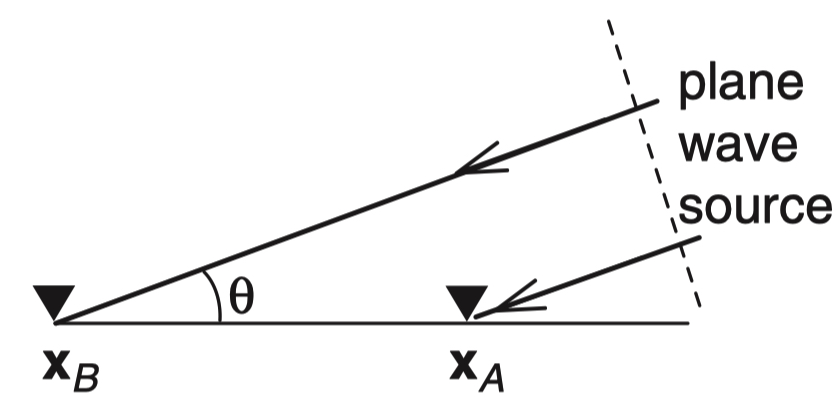
\includegraphics[width=0.6\textwidth]{noise/eg-plane-wave.jpg}
    \caption{平面波示意图}
    \label{fig:eg-plane-wave}
    \note{注:图片引自\citep{nakata2019seismic}}
\end{figure}

对于$A(\theta)$,如果其等于常数或者是随方位角变化的函数时,我们可以利用稳态法通过积分解析计算,对于其他情况我们也可以通过数值积分的方式计算。
在公式~\ref{equ:cc-pl}中存在两个稳态点,即$\theta=0°$和$\theta=180°$,
因为对于平面波我们使用高频近似假设,并假设$A(\theta)$接近于常数或者在非稳态的地方为零,我们可以简化上述积分:
\begin{align}
    C^{\pm} (x_A,x_B) \propto A_{\pm}^2 \sqrt{ \frac{2}{\pi kr} }  cos[ \omega t \mp (kr - \pi/4) ]
    \label{equ:cc-pl-cal}
\end{align}
其中$C^{\pm}$分别表示$\theta=0°$和$\theta=180°$。
对比公式~\ref{equ:gf-2d-t}和公式~\ref{equ:cc-pl-cal},我们发现互相关与格林函数之间存在下面关系:
\begin{align}
    \frac{d}{dt}C^+(x_A,x_B,t) \propto  - \omega A_+^2G(x_A,x_B,t)
    \label{equ:cc-gf}
\end{align}
相比如多模态叠加的方法,利用平面波我们添加了不同噪声源方位的约束,通过改变$A(\theta)$,我们可以通过数值积分的方法计算,来定量衡量噪声源分布的问题。


\subsection{其他背景噪声干涉}
近些年也发展了其他背景噪声干涉的原理,例如给定一个噪声点源,从表示定理出发计算该噪声源的位移场,并对整个空间上的噪声源进行积分表示完整的位移场,
我们也可以获得一致的结论,这种思路与平面波稳态的方法也是类似的,所以这里不做过多赘述。
上面所有的理论都依赖于一些“苛刻”的假设,例如噪声源均匀分布等等,这些假设通常在地球上是不存在的,人们只能通过人为经验来判断经过互相关恢复出来的格林函数是否准确。
一种替代的方法是不直接通过互相关恢复格林函数,而是把格林函数当做客观存在的时间序列,通过敏感核函数不断改变噪声源与地下结构等信息,来近似我们观测到的噪声信号,而不是直接通过干涉的方法。
这样的应用最先在太阳地震学中被提出~\citep{woodard1997implications,gizon2002time}。

我们从表示定理出发,对于波场$u$,可以通过噪声源$N$和它们之间的格林函数$G(m)$表示:
\begin{align}
    u(x_A) = \int\nolimits_{\partial D} G(x,x_A) N(x) dx
    \label{equ:u-rp}
\end{align}
将位移场$u(x_A)$与$u^*(x_B)$相乘,我们有:
\begin{align}
    u(x_A) u^*(x_B) = \iint\nolimits_{\partial D} G(x,x_A) G^*(y,x_B) N(x) N^*(y) dx dy
    \label{equ:cc-rp}
\end{align}
通常把边界$\partial D$假设为地球表面,因为噪声多数在表面上分布。当噪声源之间不存在相关性时:
\begin{align}
    C(x_A,x_B) = \langle  u(x_A) u^*(x_B)\rangle  = \int\nolimits_{\partial D} G(x,x_A) G^*(y,x_B) S(x) dx
    \label{equ:cc-rp-ave}
\end{align}
上述公式描述了互相关函数与地球模型$m$(或格林函数$G(m)$),和噪声源功率谱密度$S(x)$之间的关系。
这说明对噪声波场的建模不需要长时间的噪声波场,也不受介质性质和噪声源分布的限制。
我们可以通过比较观测的互相关$C^0(x_A,x_B)$与模拟的互相关$C(x_A,x_B)$,通过二范数优化该问题:
\begin{align}
    \lambda = \frac{1}{2} \int {[ C(x_A,x_B,\omega) - C^0(x_A,x_B,\omega) ]}^2 d\omega 
    \label{equ:cc-rp-misfit-freq}
\end{align}
使用Parseval定理,可以将待优化的方程转换到时间域:
\begin{align}
    \lambda = \frac{1}{2} \int {[ C(x_A,x_B,t) - C^0(x_A,x_B,t) ]}^2 dt
    \label{equ:cc-rp-misfit-time}
\end{align}
上述公式表明,当发生噪声源扰动$\delta S$和地球结构扰动$\delta m$,那么模拟的互相关将会出现扰动从$C$到$C+\delta C$,最后将导致误差函数出现扰动从$\lambda $到$\lambda +\delta \lambda $。
我们可以通过Fréchet方法(敏感核)将上式分成噪声源敏感核与地球结构敏感核两部分,我们可以将其写成:
\begin{align}
    \delta \lambda =  \int\nolimits_{\partial D} K_{s,ij}(x) S_{ij}(x) dx 
    + \int\nolimits_{\partial D} K_{i}(x) \delta m_i(x)  dx
    \label{equ:no-cc-misfit}
\end{align}
其中$m_i$表示任意想求的地球模型,例如P波和S波的速度,密度,衰减系数等,
示例敏感核如下:

\begin{figure}[h]
    \centering
    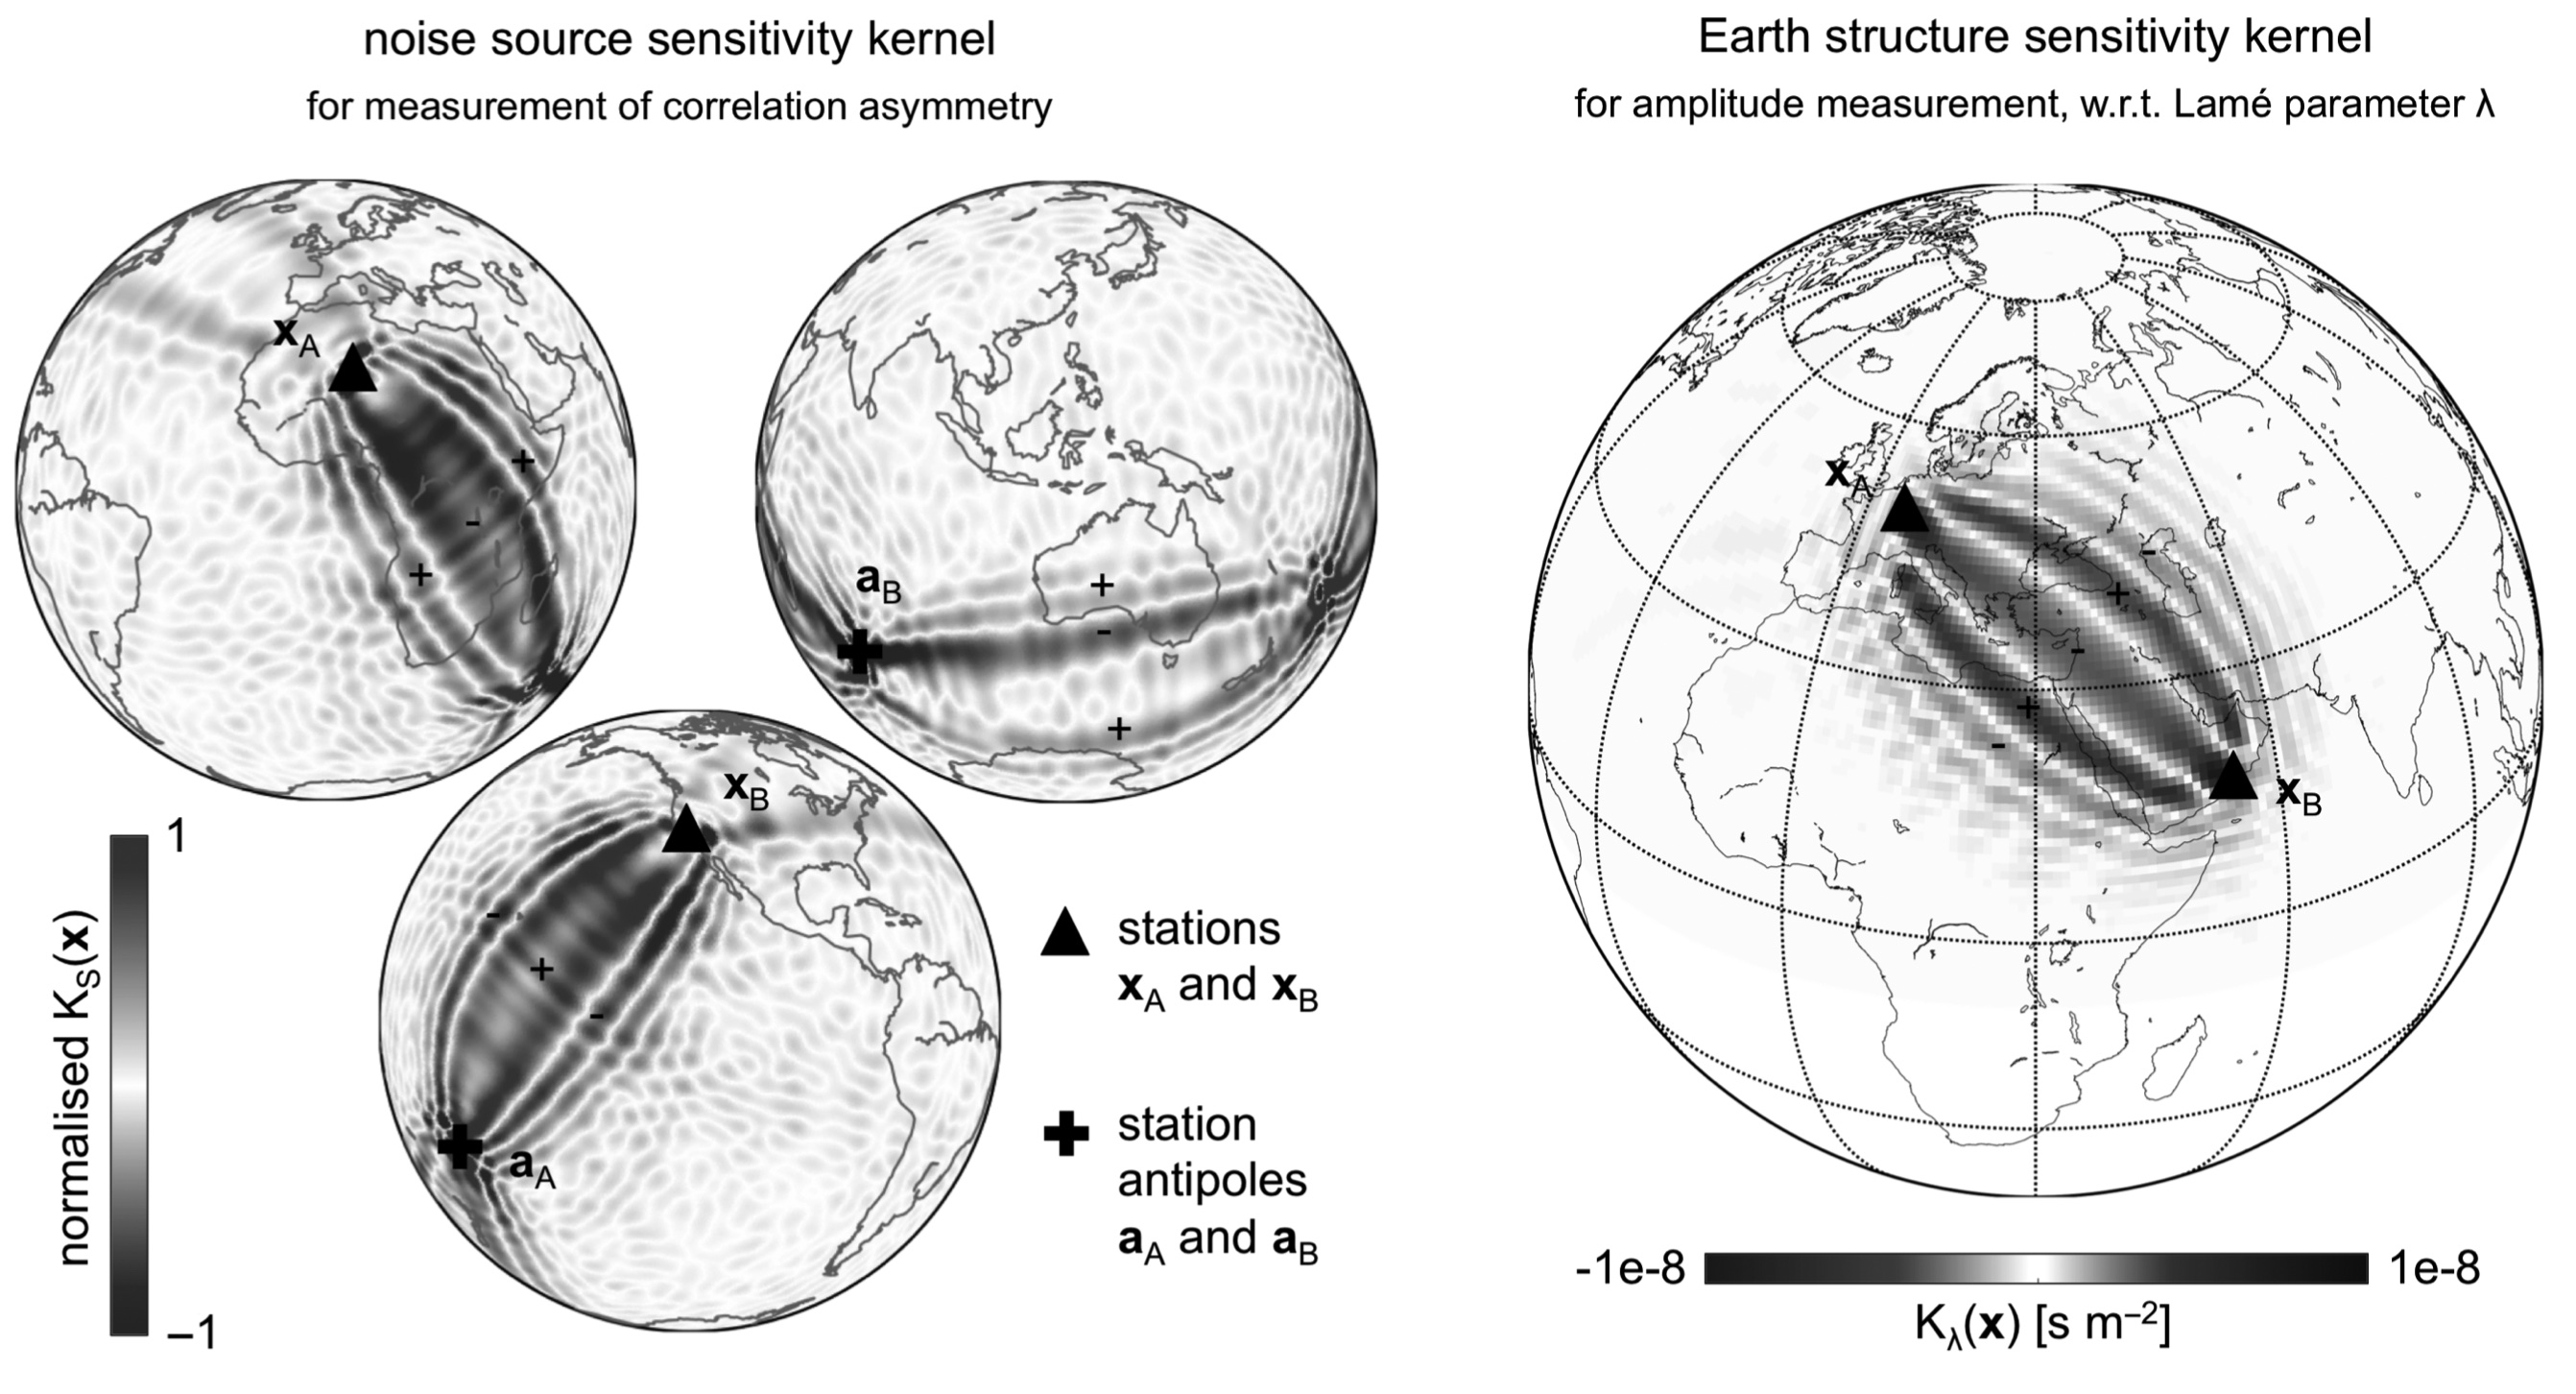
\includegraphics[width=0.95\textwidth]{noise/noise-sensitivity-kernel.jpg}
    \caption{噪声源与地球结构的敏感核}
    \label{fig:noise-sensitivity-kernel}
    \note{注:噪声源和地球结构的全球尺度敏感核。左图是长周期(150s - 300 s)面波的不对称噪声源敏感核。右图是$\lambda$长周期面波的地球结构敏感核。图片引自\citep{nakata2019seismic}}
\end{figure}

小结:在过去几十年里,背景噪声干涉技术已经深入到地震学研究的各个方向,极大提高层析成像与连续监测的分辨率;
未来高效地进行背景噪声干涉依然是研究的重点,发展不恢复格林函数的背景噪声干涉的新理论有希望在其中发挥重要作用。


\section{并行计算背景噪声互相关}


随着观测技术手段的不断提高,地震数据量越来越大,如表\ref{tab:language-parallel},
其中Seismometer表示传统地震仪,DAS表示分布式声学传感设备,Large-N表示以节点式地震仪为主的密集观测阵列,Number表示传感器数量,
Distance表示传感器的布设长度,Sample Rate表示采样率,Station Pairs表示台站对个数,Daily Size/Channel表示一天单道传感器的数据量大小,Daily total size表示一天所有传感器的数据量大小。
根据不同的观测原理与针对不同的观测目标,数据的采样频率也发现显著变化。
例如传统的地震台站仪器,通常造价昂贵,主要用来记录低频的天然地震事件,通常采样率不高,
使用的频段往往在10Hz以下,台间距往往在几十公里,一天的数据量大约在几G左右。
近些年,地震节点仪器因其造价较低廉,便携性强,越来越受地震学研究人员的青睐,大量布设的阵列能够记录更加全面的波场特征,获得更高分辨率的地下结构,它们的
采样频率与地震勘探的检波器相近,一天的数据量往往有上百G左右。
DAS仪器的出现,正改变着地震学的观测方式,其不需要购买昂贵的地震台站仪器,只需要使用现成的地下通讯光缆,就能记录形变信号。
其通过出射的光信号相位与散射相位的差异,解调生成对应位置的形变信号,也正因为需要对光信号进行记录,所有它的采样率通常较高,能够达到几千Hz。
这也意味着DAS仪器需要巨大的存储空间,其单道数据每天的大小可达几百G。

\begin{table}[h]
    \centering
    \caption{不同地震观测仪器数据特点}
    \label{tab:language-parallel}
  %   \begin{tabular}{c|cccp{6em}p{3em}c}
      \centering%把表居中
      \begin{tabular}{m{2cm}<{\centering}m{2.5cm}<{\centering}m{2.5cm}<{\centering}m{2.5cm}<{\centering}}
  
      \toprule
         & \textbf{Seismometer} & \textbf{Large-N} & \textbf{DAS}  \\
  
      \midrule
      Number &  <0.5k & 1-2k & 5-10k  \\
      \specialrule{0em}{2pt}{2pt}

       Distance & >10km & 100-1000m  & 1-10m  \\
       \specialrule{0em}{2pt}{2pt}

      Sample Rate & 20Hz & 100-500Hz & 1-10kHz  \\
      \specialrule{0em}{2pt}{2pt}

        Station Pairs & <100k  & <2000k   & <50000k \\
        \specialrule{0em}{2pt}{2pt}

       Daily Size/Channel & 7MB  & 70MB   & 70MB \\
       \rowcolor{yellow} Daily total size &  3.4G & 140G   & 680G \\

      \bottomrule
    \end{tabular}
    % \note{注:P Wave First Motion 和 CAP的结果来自中国地震局}
\end{table}


目前存在众多开源的互相关计算程序包,编写的语言、并行方式与适用范围各不相同,它们的不同特点在表~\ref{tab:cc-package}中。
其中SeisNoise.jl,NoisePy和Mirmex支持GPU运算,并且因为SeisNoise.jl的设计模式是将每个模块分开编写,需要用户自己将所有功能串联起来,所以适用性高,可使用所有种类的并行加速,便于处理各类任务。

\begin{table}[h]
    \centering
    \caption{开源的背景噪声互相关程序包}
    \label{tab:cc-package}
  %   \begin{tabular}{c|cccp{6em}p{3em}c}
      \centering%把表居中
      \begin{tabular}{m{2cm}<{\centering}m{2cm}<{\centering}m{2.5cm}<{\centering}m{2.5cm}<{\centering}m{1cm}<{\centering}}
  
      \toprule
      Package   & Language & Multiprocessing & Multithreading & GPU   \\
  
      \midrule
      SeisNoise.jl &  Julia & \surd  & \surd & \surd \\
      NoisePy & Python & \surd & & \surd \\
      Mirmex &  C++ & &  \surd & \surd \\
        CC-FJ  & Python with C++ & & \surd  & \\
        NoiseCorr & MATLAB & \surd & & \\
      \bottomrule
    \end{tabular}
    \note{注:SeisNoise.jl来自\citep{clements2021seisnoise},NoisePy来自\citep{jiang2020noisepy},Mirmex来自\citep{fichtner2017seismic},CC-FJ来自\citep{li2021cc},NoiseCorr来自\citep{yao2006surface}}
\end{table}


我们基于SeisNoise.jl~\citep{clements2021seisnoise},在Julia语言下计算背景噪声互相关。
SeisNoise.jl提供了全面的互相关计算模块,用户需要设计自己的计算流程,并编写并行程序将所有模块串联起来,实现自己特定的任务。
% Julia语言是2009年由MIT科学计算实验室发明,在2018年发布Julia 1.0.0 版本,并逐渐进入科学计算人员们的视线。
Julia语言是一门解释性(动态)语言,但其拥有近似C语言的速度(图~\ref{fig:julia})、类似MATLAB一样方便的矩阵运算、
像shell语言一样能够将不同语言的代码粘合在一起,并且拥有强大的并行计算库,目前越来越多的科学计算工作转向Julia语言。
图 ~\ref{fig:julia} 表示了不同语言的测试速度,参与测试与语言版本为Julia v1.0.0, SciLua v1.0.0, Rust 1.27.0, Go 1.9, Java 1.8.0, Javascript V8 6.2.414.54, Matlab R2018a, Anaconda Python 3.6.3, R 3.5.0, Octave 4.2.2., C 与 Fortran 是使用 gcc 7.3.1 进行编译。

目前国内基于Julia语言的地震学研究还很有限,国外的研究于近几年刚刚起步,目前Julia语言地震学程序包的开发还是以研究者个人为主,以组织或研究组的开发团队还较少,
天然地震的程序开发组有来着哈佛大学的 \href{https://denolle-lab.github.io/}{Denolle Quake Lab} 课题组,主要开发天然地震数据的读取与处理、常规地震数据处理流程、背景噪声干涉互相关程序等。
勘探地震的程序开发组有来自佐治亚理工的 \href{https://slim.gatech.edu/}{Seismic Laboratory for Imaging and Modeling}课题组,其与微软公司合作,主要面向于下一代地震勘探即以人工智能与云计算与主导的地震勘探技术。

\begin{figure}[h]
    \centering
    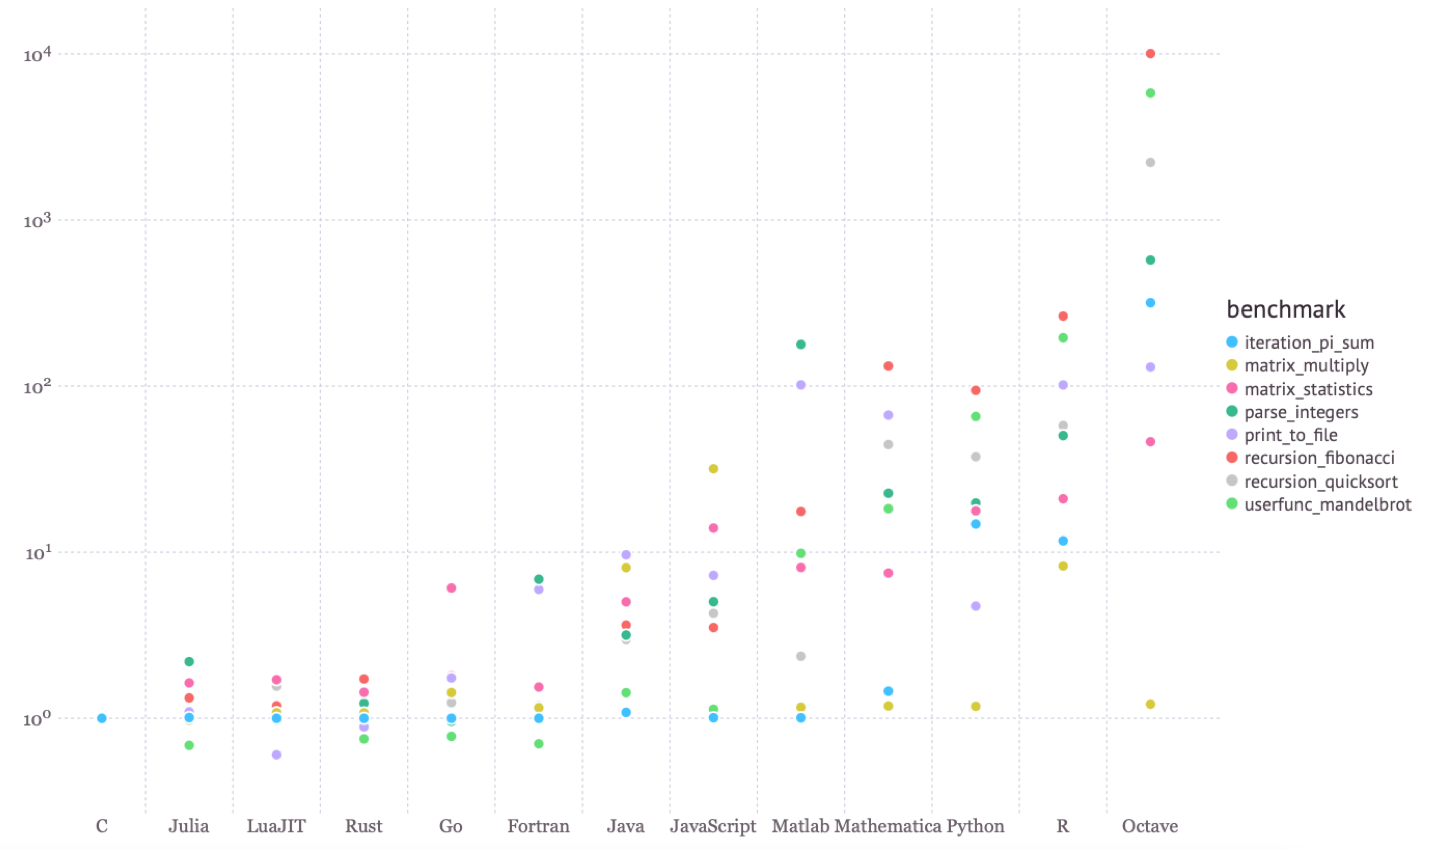
\includegraphics[width=0.9\textwidth]{noise/julia.png}
    \caption{不同语言的运行速度比较}
    \label{fig:julia}
    \note{注:纵轴是以C语言为基准的运行时间,测试硬件信息为Intel core i7-3960X 3.30GHz CPU、64GB 1600MHz DDR3 RAM、Linux,图片引自\href{https://julialang.org/benchmarks/}{Julia官网。} }
\end{figure}

% ,上述测试是在用Julia v1.0.0、SciLua v1.0.0-b12、Rust 1.27.0、Go 1.9、Java 1.8.0_17、Javascript V8 6.2.414.54、Matlab R2018a、Anaconda Python 3.6.3、R 3.5.0和Octave 4.2.2中进行计算测试。,


我们遵循Bensen提出的背景噪声处理流程\citep{bensen2007processing},先将连续的地震数据进行分段(通常按照天),对每一段数据去除仪器响应、去除均值趋势,
进行带通滤波;然后进行时间域归一化,变换到频率域内再进行谱白化,确保各频率成分相同;然后进行互相关运算,变换到时间域后进行多次叠加。
我们使用Julia语言下的多进程与多线程并行技术,针对目前常见的背景噪声干涉应用领域,噪声频散成像与波速变化监测,设计了互相关并行运算框架,如图~\ref{fig:cc-flow},该框架的数据处理模块依赖于SeisNoise.jl。
根据计算机内存是否满足一次性读取所有地震数据的能力,我们将其分为两种模式,直接进行傅里叶变换与互相关运算,然后叠加;或者先进行傅里叶变化,然后将频率域数据保存,再进行互相关运算,最后再叠加。
并行计算时的线程数与进程数可根据计算资源设置,一般情况下使用的核心数越多,计算速度越快。
后面我们的互相关运算都依赖于此程序。关于该程序的详细使用说明请参见网站:\href{https://github.com/OUCyf/NoiseCC}{https://github.com/OUCyf/NoiseCC}。

\begin{figure}[h]
    \centering
    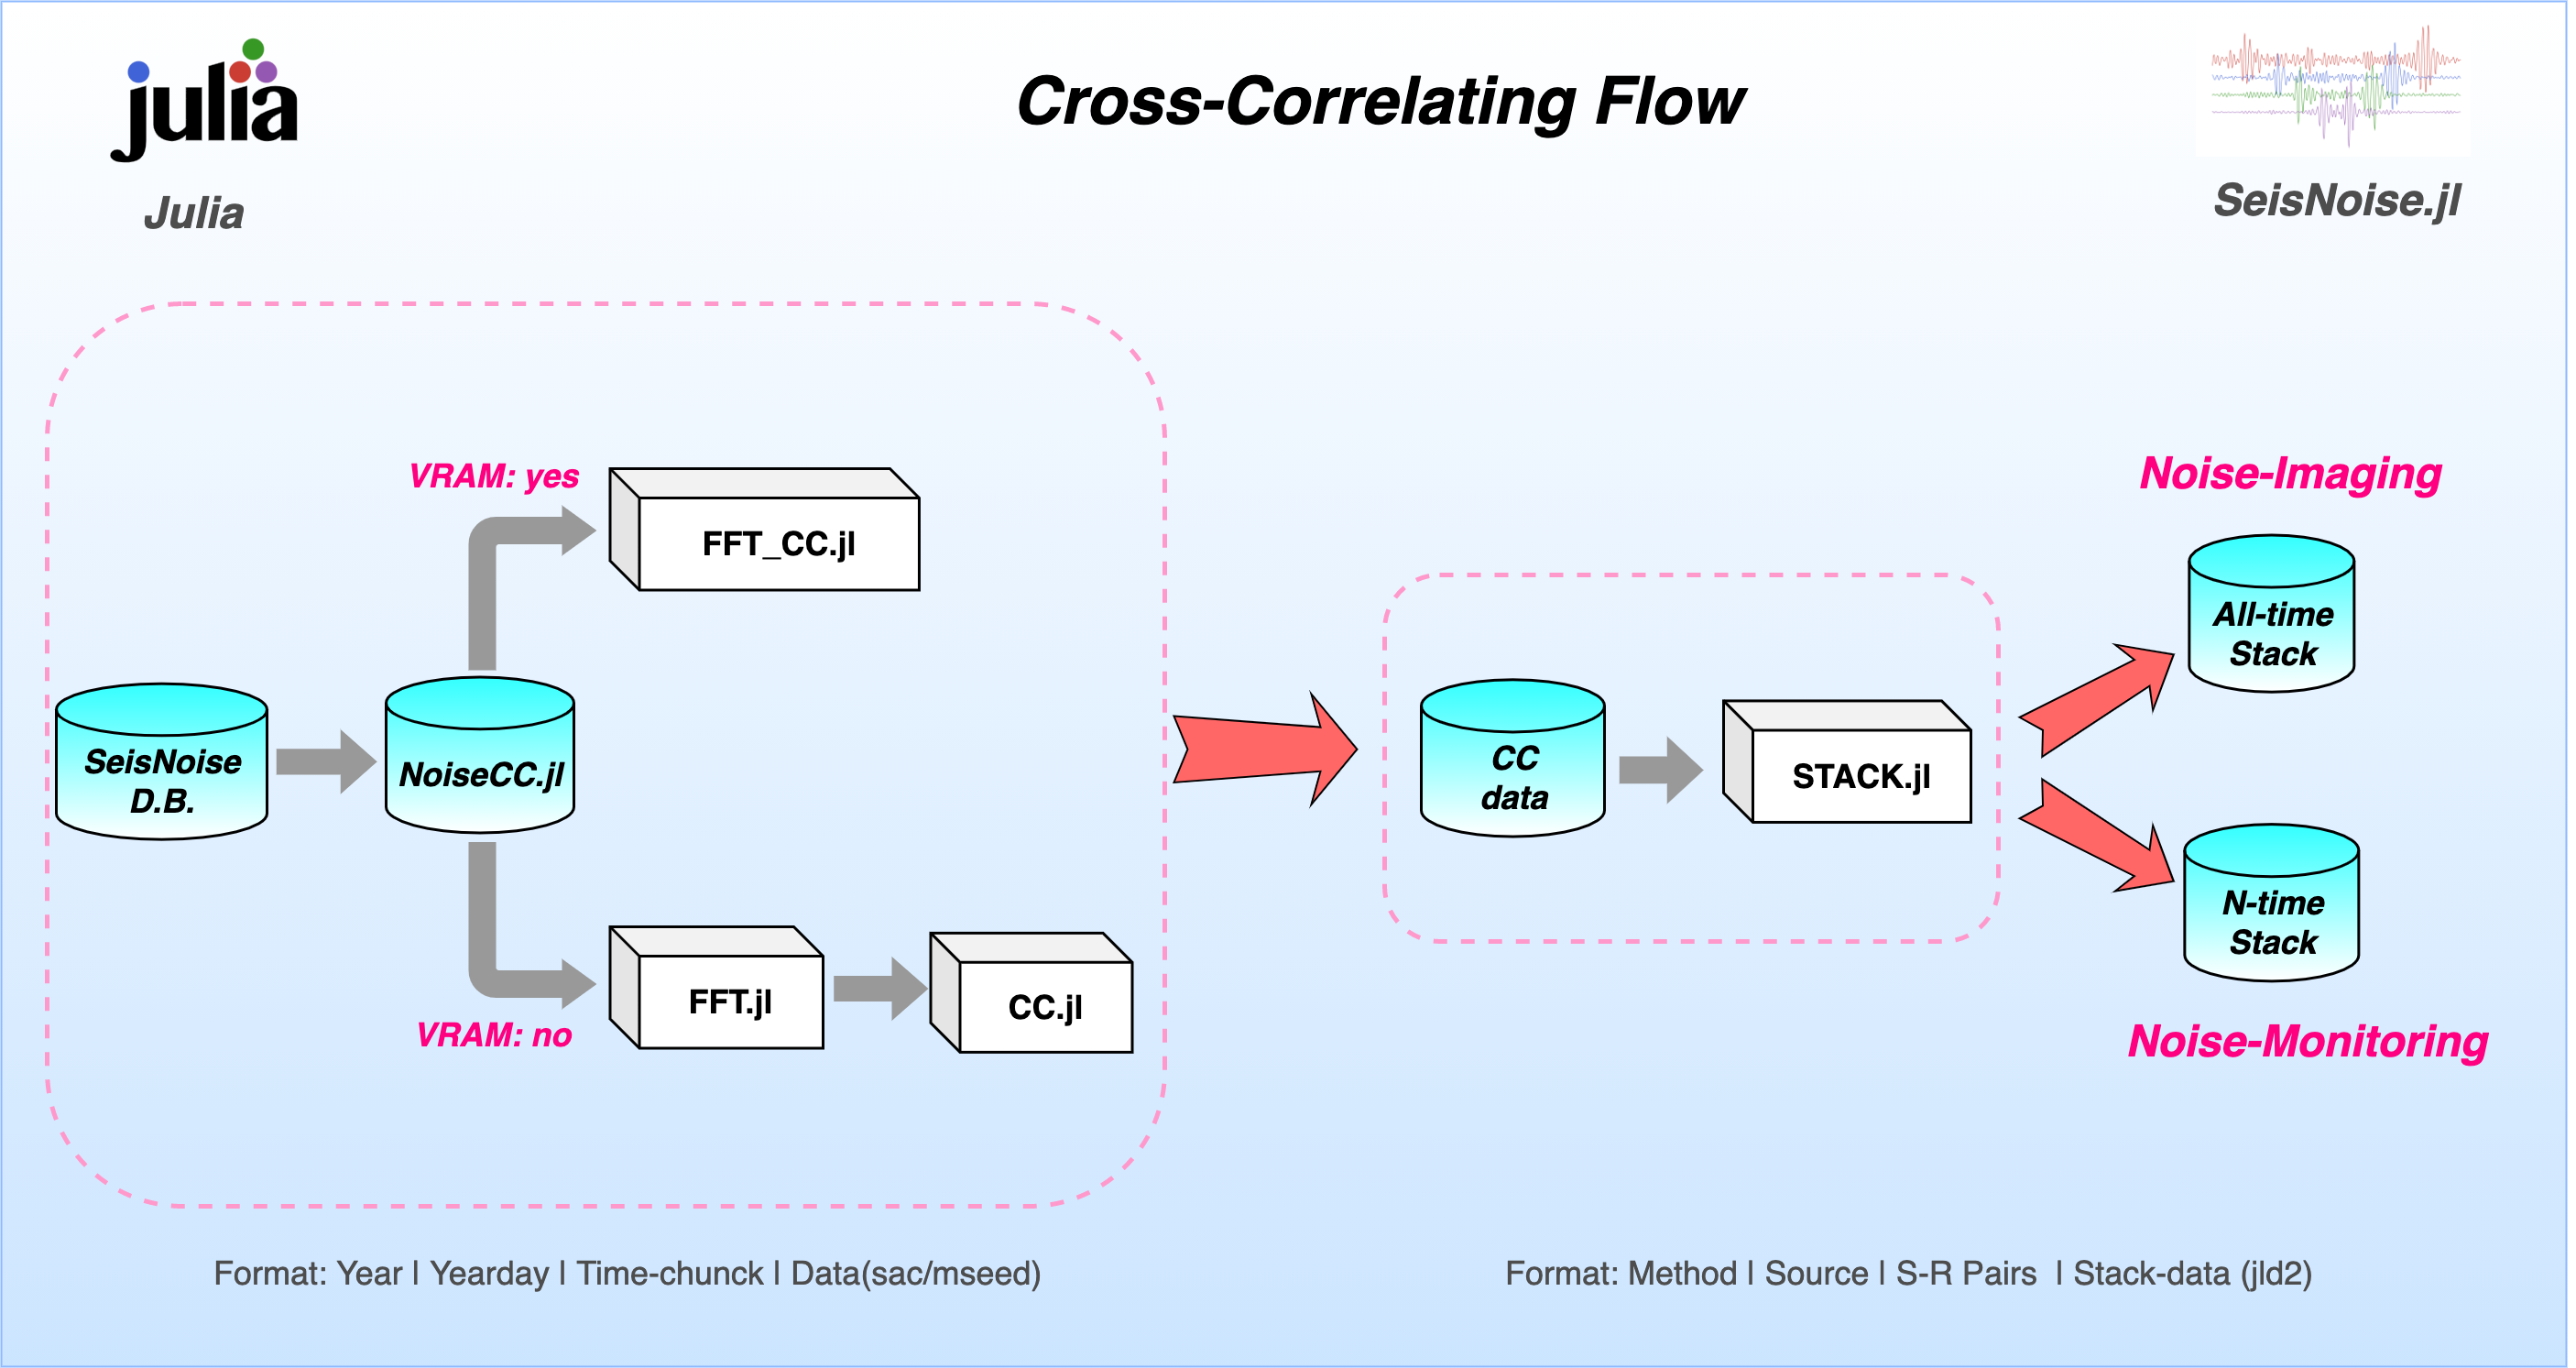
\includegraphics[width=0.9\textwidth]{noise/cc-flow.png}
    \caption{NoiseCC 程序的流程图}
    \label{fig:cc-flow}
    % \note{注:图片引自\href{https://julialang.org/benchmarks/}{Julia官网} }
\end{figure}



% \chapter{背景噪声在DAS成像中的应用}


\section{DAS传感技术}

\begin{figure}[h]
    \centering
    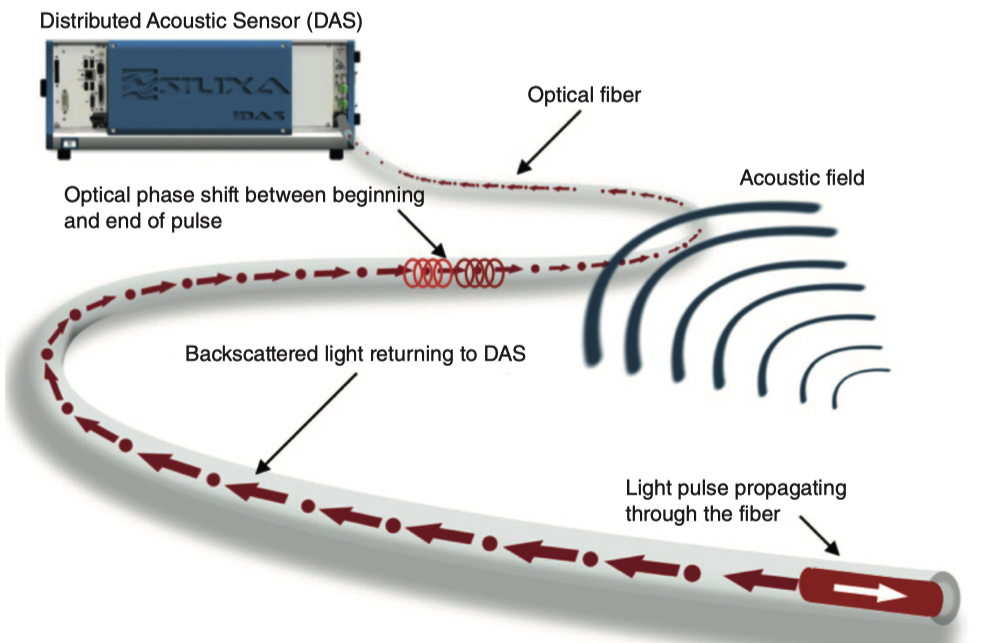
\includegraphics[width=0.85\textwidth]{imaging/das-equipment.jpg}
    \caption{分布式声传感的工作原理}
    \label{fig:das-equipment}
    \note{注:图片引自\citep{li2022distributed}}
\end{figure}

分布式声学传感技术,Distributed Acoustic Sensing(DAS),是一项最近十年兴起的地震观测技术,见图~\ref{fig:das-equipment}。
它可以使用普通的光纤电缆记录振动信号,细如发丝的玻璃纤维就是它的传感器。
光纤内部天然存在的缺陷可作为地下振动信号的应变计,这些缺陷是由于光纤的制作过程中掺入了一些杂质形成散射体造成的,见图~\ref{fig:das-scatter}。
DAS的基本工作原理是,通过向光纤中发射脉冲光,测量背向散射光的相位差,并据此得到光纤沿线的应变率。
大多数DAS仪器利用瑞利散射原理来测量应变率。


\begin{figure}[h]
    \centering
    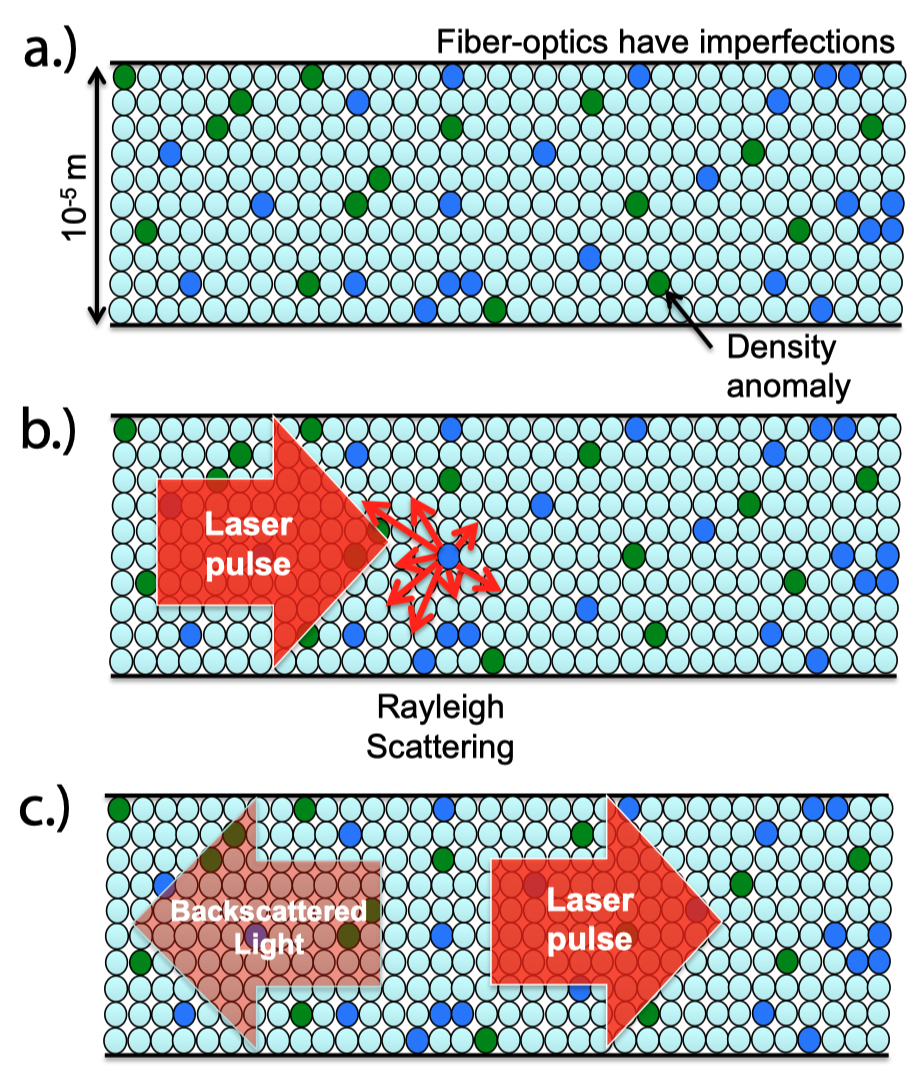
\includegraphics[width=0.85\textwidth]{imaging/das-scatter.jpg}
    \caption{DAS测量原理概念图}
    \label{fig:das-scatter}
    \note{注:(a)普通的单模光纤电缆芯因制造杂质而产生密度波动;(b)相干激光脉冲在任何密度变化下都会发生瑞利散射;(c)当激光脉冲沿着光纤继续传播时,背向散射光返回到探测器。
图片引自\citep{lindsey2019fiber}}
\end{figure}


光信号的解调方式有两种,时间域解调与频率域解调。测量的相位差与沿光纤方向的应变存在以下关系,

\begin{equation}
    \epsilon  = \frac {\Delta L} {L} = \Delta \theta \frac {\lambda } {L}
    \label{equ:strain-phase}
\end{equation}

其中$\epsilon$表示应变,$L$是计算应变时选择的测量长度(Gauge-Length),$\Delta \theta$是解调仪计算的相位差。
$L$参数的选取会影响数据的空间分辨率,较大的$L$会降低空间分辨率,反之亦然。
一个简单的示意图如图 ~\ref{fig:das-ll}所示,未发生应变(蓝色)和发生应变(红色)之间的相位差,与该部分光纤对应的应变成正比。

\begin{figure}[h]
    \centering
    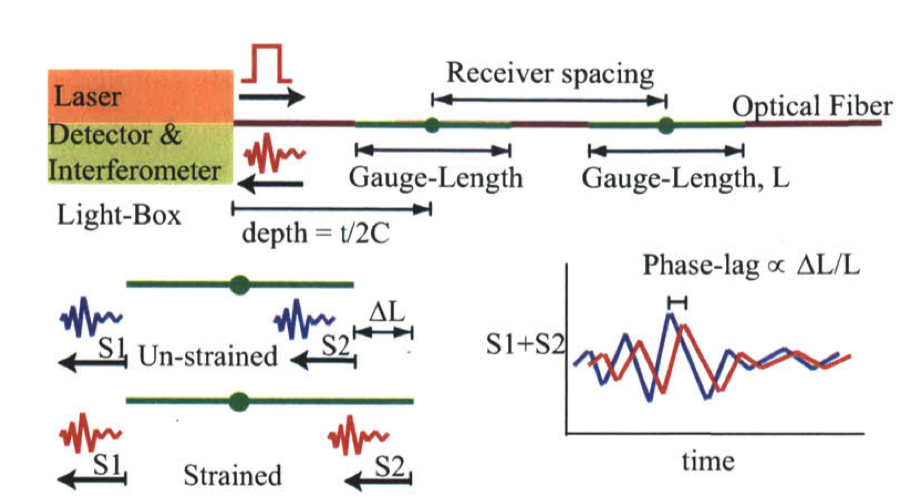
\includegraphics[width=0.85\textwidth]{imaging/das-ll.jpg}
    \caption{DAS系统各组成部分的示意图描述}
    \label{fig:das-ll}
    \note{注:光纤中两个散射点在未发生应变(蓝色)和发生应变(红色)状态下形成的拍频信号(S1+S2)之间的相位滞后,其与两次采样时刻之间的光纤应变成正比。
    图片引自\citep{bakku2015fracture}}
\end{figure}

在全球现有的光缆中未使用的光纤(暗光纤)很常见,因其可以使用现有光纤网络,所以它以极低的价格大大扩展了现有地震监测网络。
光纤长度可以长达数十公里,每隔几米的位置就可以对地震动信号进行采样。
DAS阵列在区域地震学可以应用于三大领域:地震监测、断层和许多其他地质构造的成像以及灾害评估\citep{zhan2020distributed}。
近些年DAS阵列野外的实验结果表明,其具有超宽频带、高保真度波形信号和超高分辨率\citep{ajo2019distributed}。


利用地震波对地下结构成像,为我们理解地震孕育过程、地下流体性质和预测强地面运动等工作,是非常重要的。
在某些地区,例如断层带、盆地周边等,它们拥有着强烈的横向不均匀性,速度变化差异极大,传统的地震台站间距通常较大,无法对剧烈变化的地下结构进行高分辨率成像。
道间距为1-10米的密集DAS阵列,能够有效捕捉这些地区的地震波场特征。
PoroTomo项目利用布设的8000个DAS通道,分析重型卡车激发的信号,获得了几百米深的土壤和基岩高分辨率速度图像\citep{parker2018active}。
但与传统地震仪的数据相比,DAS传感器具有指定方向的灵敏度,使得DAS的噪声干涉成像更加具有挑战性\citep{martin2021introduction}。
到目前为止,因为数据量巨大导致存储困难,大多数DAS网络都是临时部署的,所以没有探测到足够的地震,还没有获得区域尺度上的深层结构。
但也有一些尝试性工作,Yu等人\citep{yu2019potential}从DAS阵列中捕获了远震信号,从面波中提取出10-50s频散信息,
借助DAS阵列周边的台站,演示了利用DAS进行远震p波接收函数工作的可能性。


长时间布设的DAS阵列可以监测地下的变化。
Dou等人\citep{dou2016surface}使用DAS阵列监测阿拉斯加冻土融化期间的背景噪声。
Ajo-Franklin等人\citep{ajo2019distributed}在萨克拉门托DAS阵列上,通过噪声干涉测量法进行了三个多月的高重复性监测,并计划使用它来监测地下水水位变化。
此外在4D勘探地震学中,借助小型重复震源,利用DAS可以有效地监测地热田等地区的地下变化。


% \section{提取频散的方法}

% \subsection{相移法}






% \subsection{F-J变换法}




\section{2020北京白家疃DAS实验}

\subsection{实验简介}
在城市地区进行地震观测,对于城市地下空间规划建设与抗震减灾有着重要的指导意义。
通常精细的地下空间结构探测依赖于高密度的台阵布设,但在人口密集的城市地区进行高密度台阵布设往往充满困难。
分布式光纤传感技术(DAS)作为一种新的地震观测手段,为低成本高密度台阵布设提供了新的解决方案。
2020年国庆期间,我们在北京进行连续十天的DAS观测实验,使用来自上海朴牛有限公司的解调设备。
总长约1公里的实验光缆,被分成260个独立观测单元,道间距4米,所有的光纤布设在地下约30cm深的位置,与土层耦合良好。
期间进行了80次人工落锤实验,见图\ref{fig:baijiatuan-map}。
十天的观测实验总共获得近20T的原始数据,从降采样处理后的地震记录中可识别出人工落锤信号、天然地震信号与周边干扰噪音。
利用背景噪声互相关技术提取的面波信号,可以获得地下浅层S波速度结构剖面。
以上初步实验结果表明光纤传感技术在将来城市空间探测中将会发挥重要作用。

\begin{figure}[h]
    \centering
    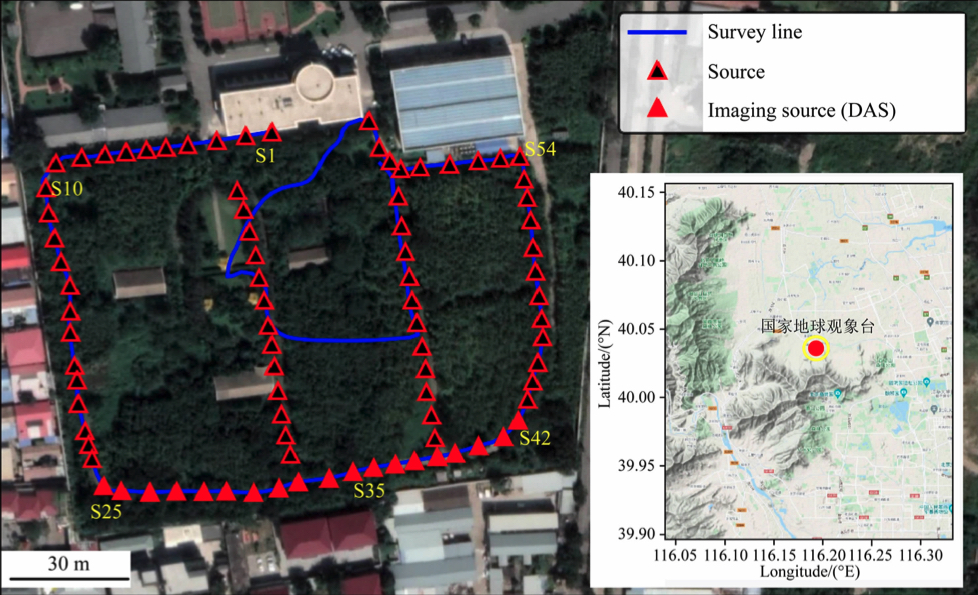
\includegraphics[width=0.85\textwidth]{imaging/baijiatuan-map.jpg}
    \caption{白家疃DAS阵列观测系统}
    \label{fig:baijiatuan-map}
    \note{注:红色三角形为人工震源位置,红色实心三角形为本次研究区域,蓝色曲线是光纤布设位置。图片引自\citep{lei2021shallow}}
\end{figure}


在本次实验中,我们成功监测到了多种信号,如图~\ref{fig:earthquake}。
其中包括122km远处的一次3级左右的小地震事件,可以清晰地看到P波与面波的信号,地震信号的主频在10Hz以下。
在P波到来前,可以看到一个移动的噪声源信号,是汽车经过产生的噪声,粗略估计它的视速度大约43$km/h$。
此外,在P波与面波之间,还能清晰地看到一次人工落锤记录的信号。

\begin{figure}[h]
    \centering
    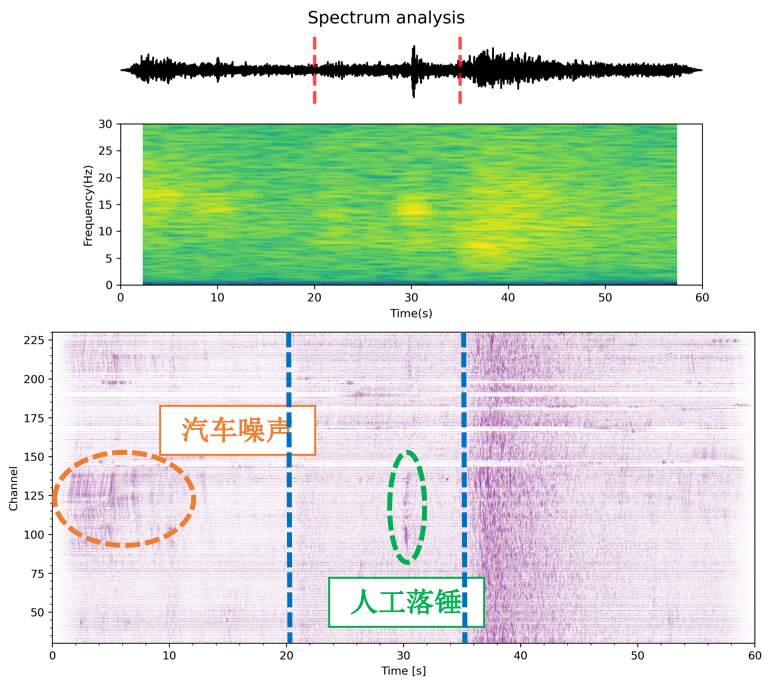
\includegraphics[width=0.85\textwidth]{imaging/earthquake.png}
    \caption{2020年10月21日,震中距约为122km的小地震记录}
    \label{fig:earthquake}
    % \note{注:红色三角形为人工震源位置,红色实心三角形为本次研究区域,蓝色曲线是光纤布设位置。图片引自\citep{lei2021shallow}}
\end{figure}









\subsection{背景噪声频散成像}

我们将DAS阵列中第50道,在2022年10月4日一整天的噪声信号绘制出来,如图~\ref{fig:noise-one-day}。
分析发现,该信号存在严重的单频干扰(24.5Hz),分别出现在早上7点-8点之间、中午10点-11点之间、和傍晚4点-5点之间,
分析单频信号发生的位置,位于白家疃北京国家地球观象台的食堂区域,推测是由于食堂中某些单频设备造成的干扰信号。
此外还能看到持续一整天的人工落锤信号。

\begin{figure}[h]
    \centering
    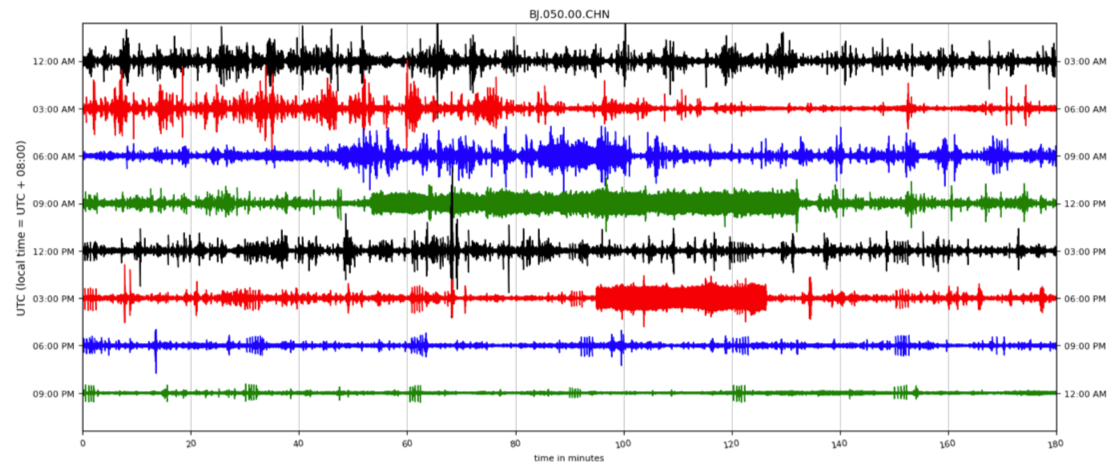
\includegraphics[width=0.85\textwidth]{imaging/noise-one-day.png}
    \caption{DAS第50道在2020年10月4日的噪声记录}
    \label{fig:noise-one-day}
    % \note{注:红色三角形为人工震源位置,红色实心三角形为本次研究区域,蓝色曲线是光纤布设位置。图片引自\citep{lei2021shallow}}
\end{figure}

在去除这些信号后,我们选取DAS阵列的南侧通道(从S25到S42,见图\ref{fig:baijiatuan-map}),进行背景噪声互相关运算。
我们遵循Bensen提出的流程,把选取的通道数据截成1分钟每段,进行0.5Hz-22Hz带通滤波,在时间域剔出振幅较大的异常信号,并在频率域进行谱白化处理,然后进行互相关运算,
并使用相位加权的方法在时间域进行叠加,最终的互相关信号如图~\ref{fig:cc-waveform}。


\begin{figure}[h]
    \centering
    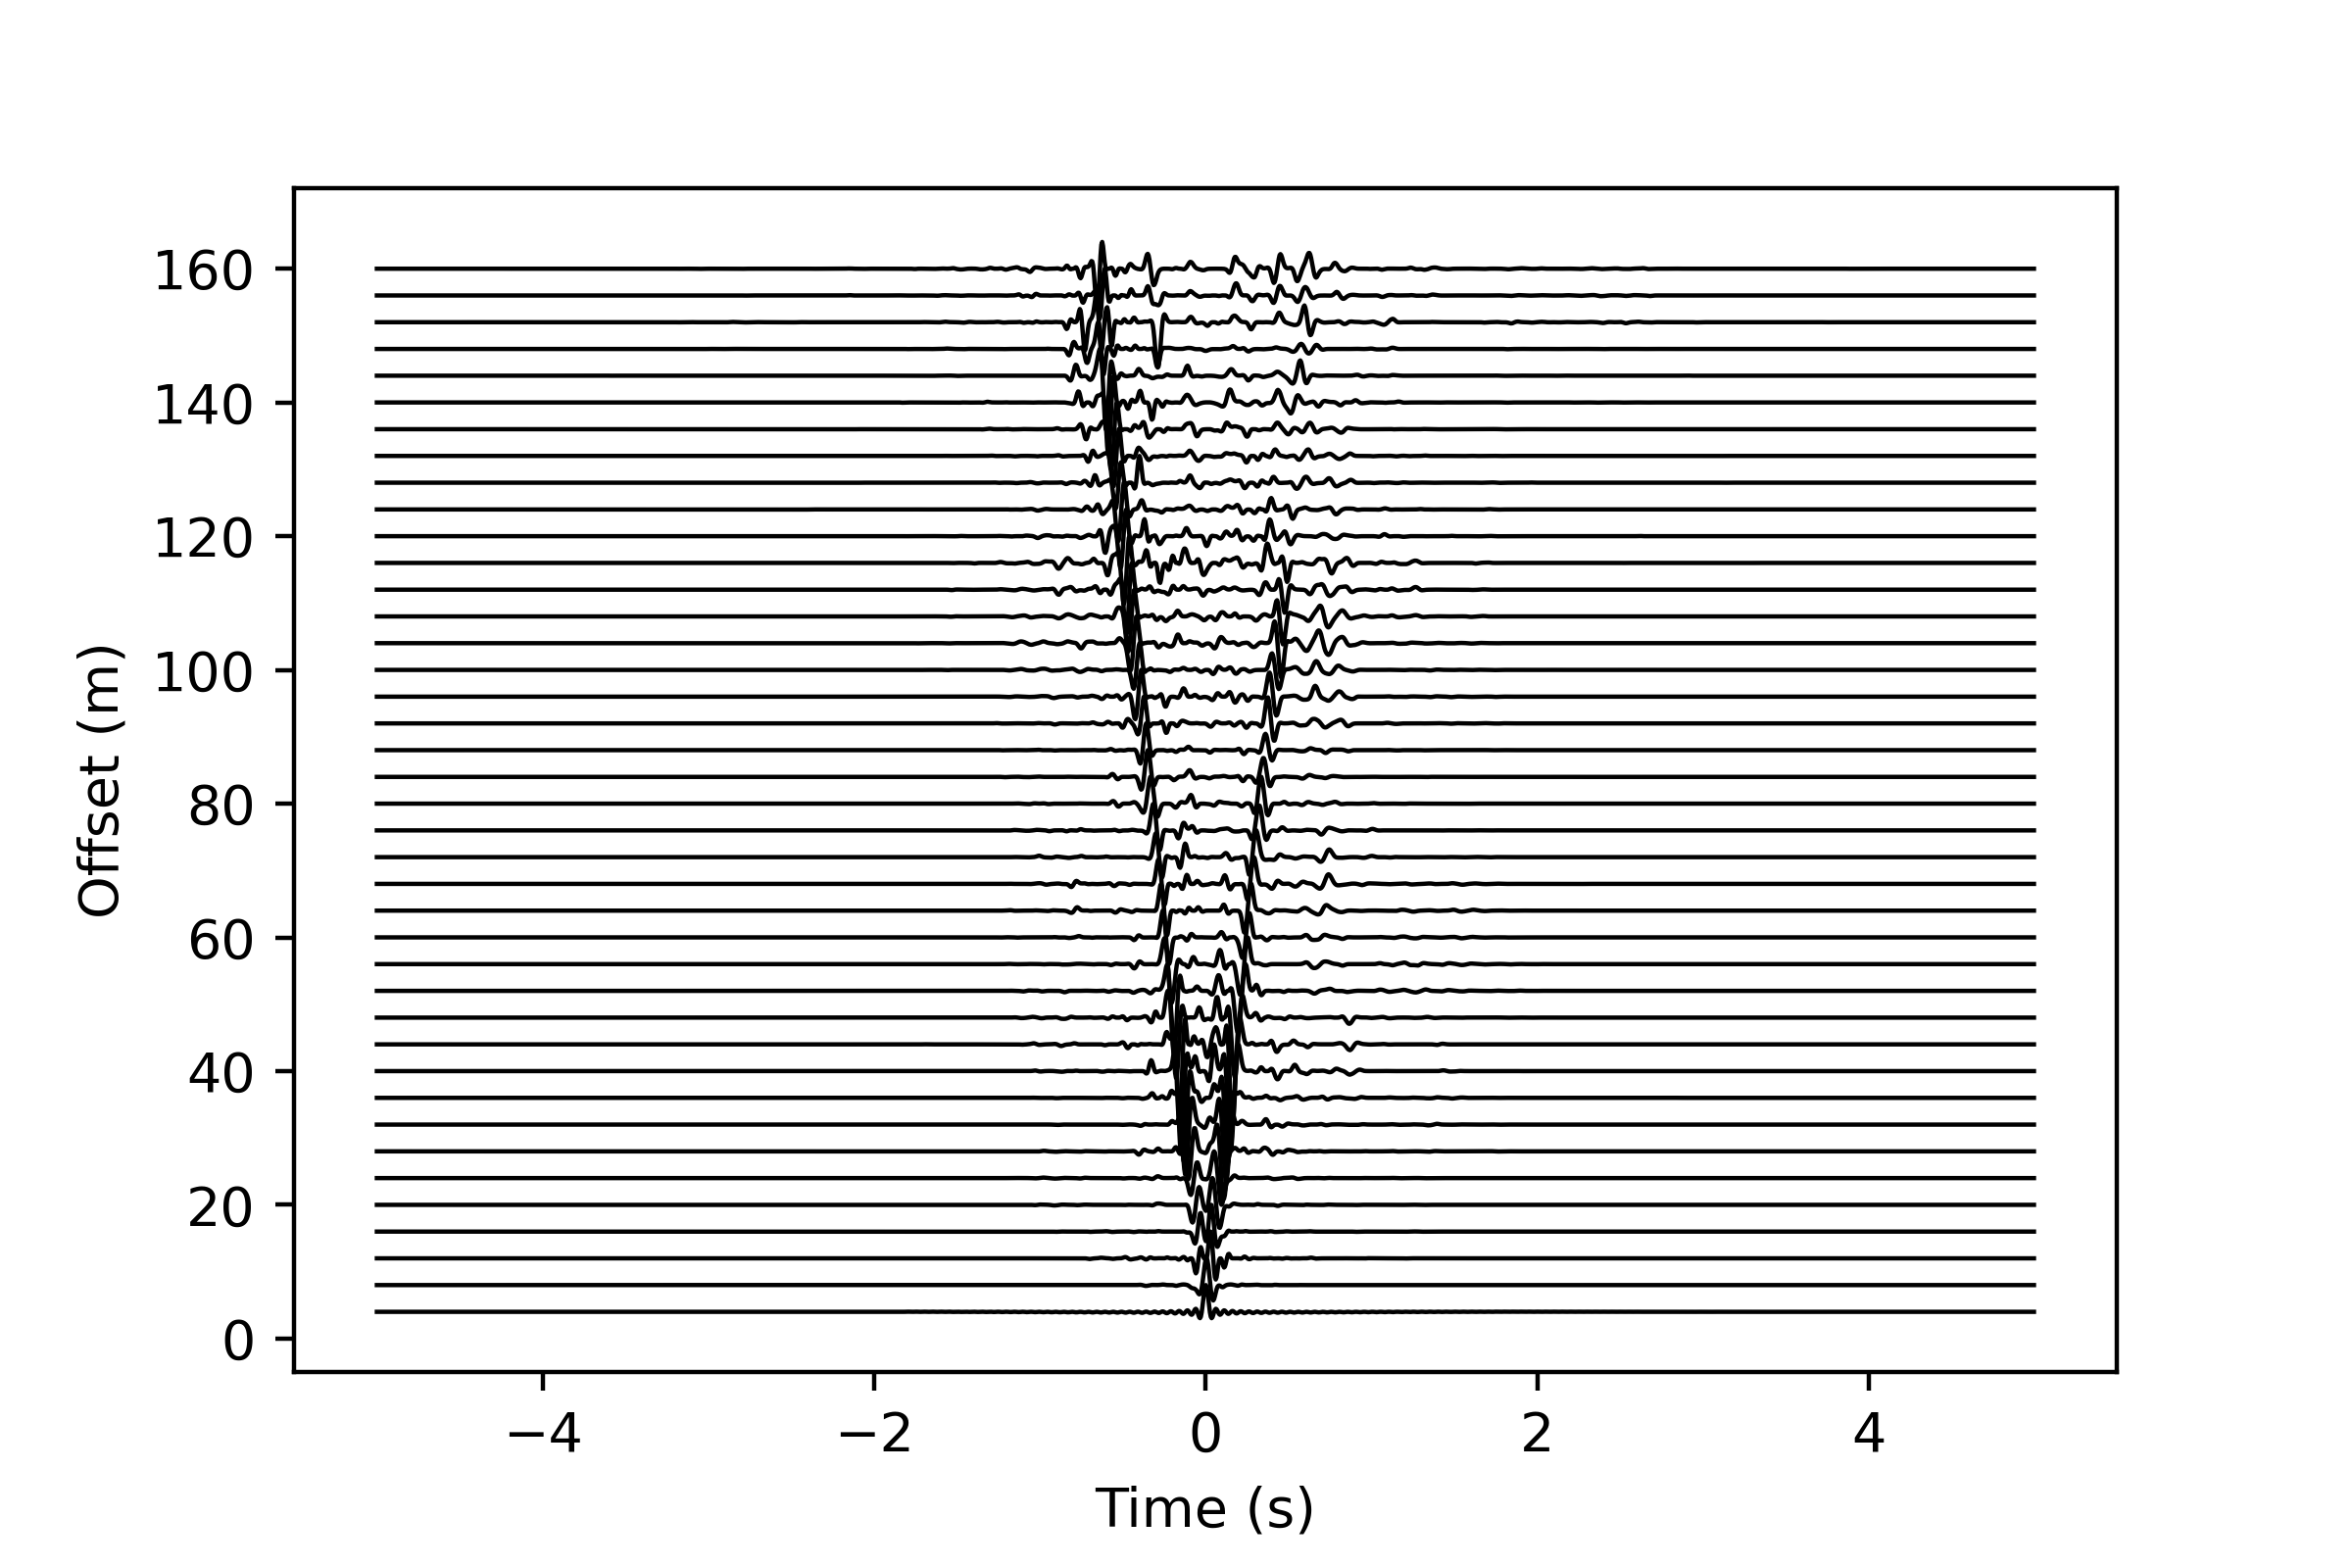
\includegraphics[width=0.85\textwidth]{imaging/cc-waveform.png}
    \caption{背景噪声互相关结果}
    \label{fig:cc-waveform}
    % \note{注:红色三角形为人工震源位置,红色实心三角形为本次研究区域,蓝色曲线是光纤布设位置。图片引自\citep{lei2021shallow}}
\end{figure}


我们基于多道面波分析(MASW),利用相移法对互相关结果进行相速度测量,该方法基本原理如下。
首先将时间域的互相关记录$d(x,t)$变换到频率域:
\begin{align}
    u(x,f) =   \int\nolimits_{-\infty}^{\infty} d(x,t) e^{-i2\pi ft} dt
    \label{equ:fft}
\end{align}
通过给定相速度$c$计算距离$x$的相移,并对所有记录数据进行叠加,获得频率$f$和相速度$c$能量的图像,最大能量点即为频散曲线:
\begin{align}
    v(\psi ,f) =   \int\nolimits_{x_0}^{x_1}  e^{-i\psi } \bigl[ \frac{u(x,f)}{|u(x,f)|}   \bigl] dx
    \label{equ:c-dispersion}
\end{align}

使用上述方法我们获得了频散曲线能量图~\ref{fig:dispersion},我们能够看到较为清晰的基阶频散的信号,
其低频信号能够到达3Hz左右。


\begin{figure}[h]
    \centering
    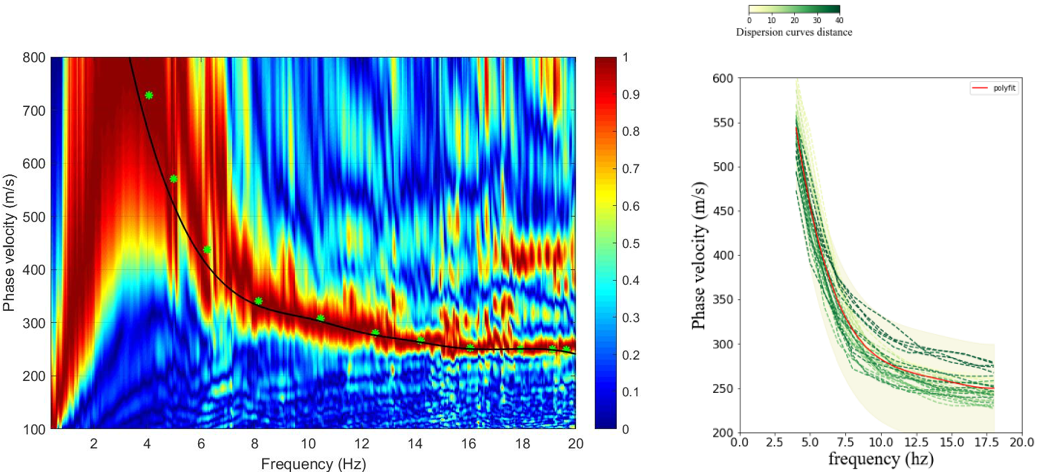
\includegraphics[width=0.85\textwidth]{imaging/dispersion.png}
    \caption{相速度频散曲线}
    \label{fig:dispersion}
    \note{注:相速度频散曲线,右边子图是整个区域所有的频散曲线,红色线表示平均相速度频散曲线。}
\end{figure}


我们通过移动虚拟震源和排列,反演它们中点下方的层状速度结构,最后将所有点的速度结构拼接成一个二维速度剖面。
采用阻尼最小二乘的反演方法,使用CPS\citep{herrmann2002computer}中的surf96程序进行反演,
根据Rayleigh波最大敏感深度的经验关系,我们设置本次反演的最大深度为100米,固定层厚,只反演S波速度,其中最浅层厚度为10米,往深度逐渐增加。
只使用基阶频散进行反演,层速度反演结果见图~\ref{fig:inversion},将所有的层速度拼接成二维速度剖面如图~\ref{fig:2d-velocity}。

从反演结果我们发现频散曲线的拟合结果较好,速度模型显示该区域速度呈现随深度逐渐增加的趋势,
浅部的速度大约250-300$m/s$,深度100米处的速度能够接近800$m/s$。
该结果也与2018年在同一区域进行光纤被动源实验结果较为一致~\citep{林融冰2020}


\begin{figure}[h]
    \centering
    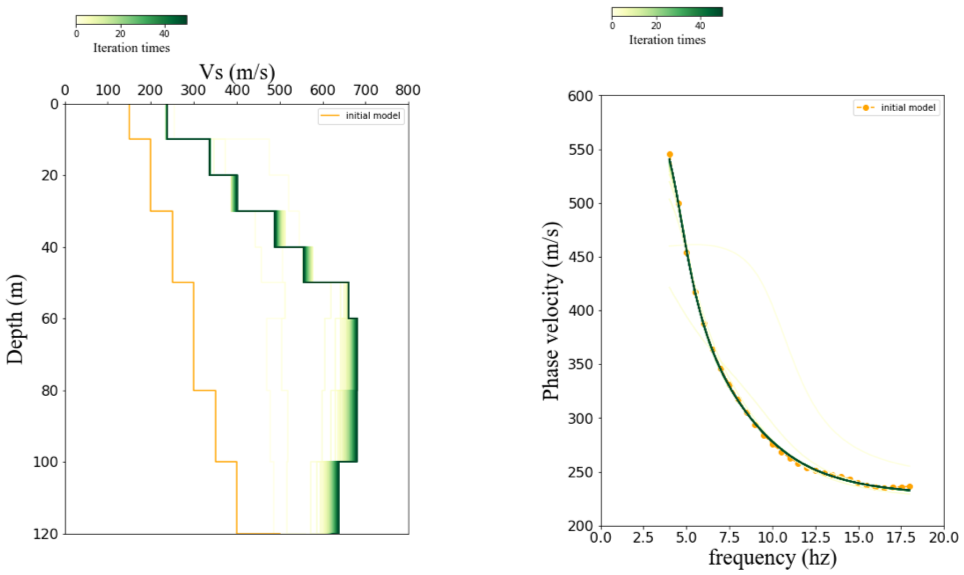
\includegraphics[width=0.85\textwidth]{imaging/inversion.png}
    \caption{层速度反演结果}
    \label{fig:inversion}
    \note{注:左面子图的黄色折线是初始速度模型,绿色渐变线是不同迭代次数的反演速度模型。右边子图黄色点是观测的频散曲线,绿色曲线是反演的频散曲线。}
\end{figure}

\begin{figure}[h]
    \centering
    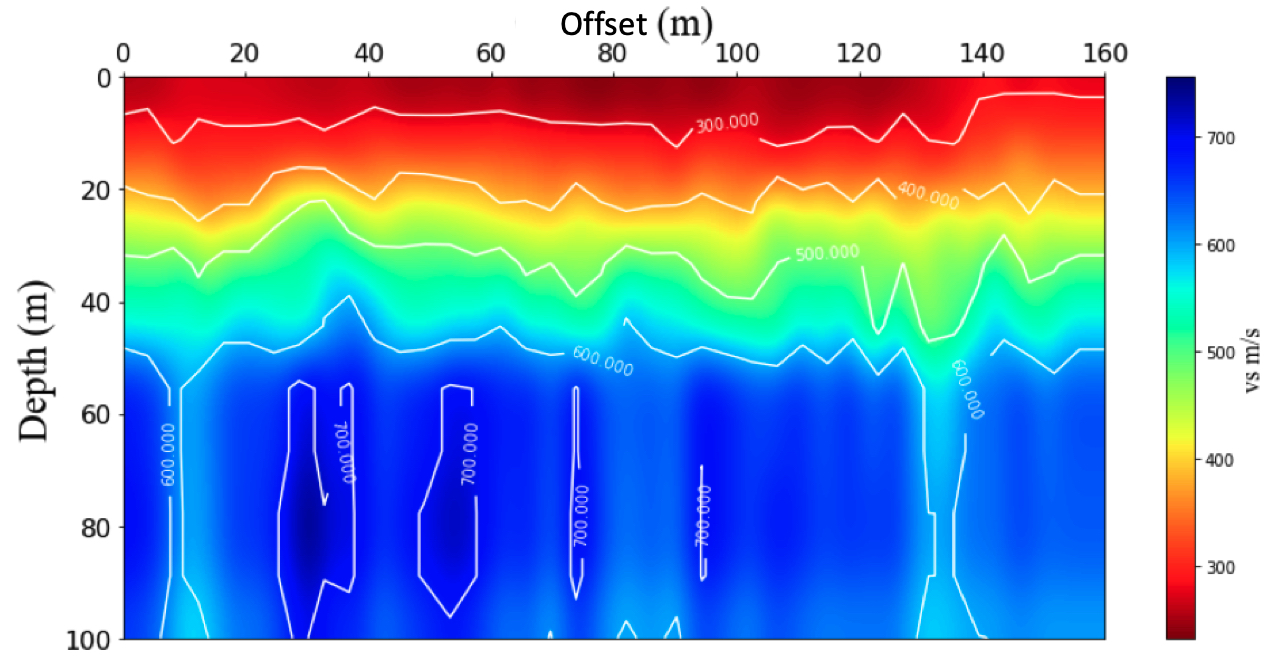
\includegraphics[width=0.85\textwidth]{imaging/2d-velocity.jpg}
    \caption{S波二维速度剖面}
    \label{fig:2d-velocity}
    % \note{注:红色三角形为人工震源位置,红色实心三角形为本次研究区域,蓝色曲线是光纤布设位置。图片引自\citep{lei2021shallow}}
\end{figure}



\section{讨论}

在上述过程中,我们使用背景噪声干涉结果中的基阶频散信号进行S波速度结构的反演,获得了一个S波速度随深度逐渐增加的结果,其中初始速度模型是根据人为经验给定的。
在研究城市浅地表区域的速度结构时,往往没有前人研究的经验,很难获得一个较为可靠的初始速度模型。
并且浅地表区域的局部速度变化差异较大,这给我们的反演工作带来了巨大困难。
针对同一批数据,我们使用主动源面波信号,利用频率贝塞尔变换的方法,提取出了高阶面波频散信号,见图~\ref{fig:fj-dispersion}。
使用基于遗传算法的全局优化方法进行反演,最终反演结果发现在30米深处存在一个高速层,见图~\ref{fig:2d-velocity-fj}。
关于主动源高阶面波成像的详细工作请参见Lei的文章\citep{lei2021shallow}。
我们发现主动源提取的基阶频散信号与我们背景噪声获得的基阶频散信号较为一致。

这说明仅使用基阶面波频散信号进行反演是不可靠的,容易陷入局部极小值,高阶信息的加入可以有效约束反演问题中多解性的问题。
基于最小二乘的反演方法往往需要一个较好的初始速度模型,反之容易陷入局部极小值。
全局优化的方法是非常必要的,其能够有效突破局部极小值的限制,搜索到全局最小值,但其代价是相应的反演时间增加。
在未来的研究中,有效提取高阶面波频散信息,开发高效率的全局优化方法,是DAS成像工作的关键。


\begin{figure}[h]
    \centering
    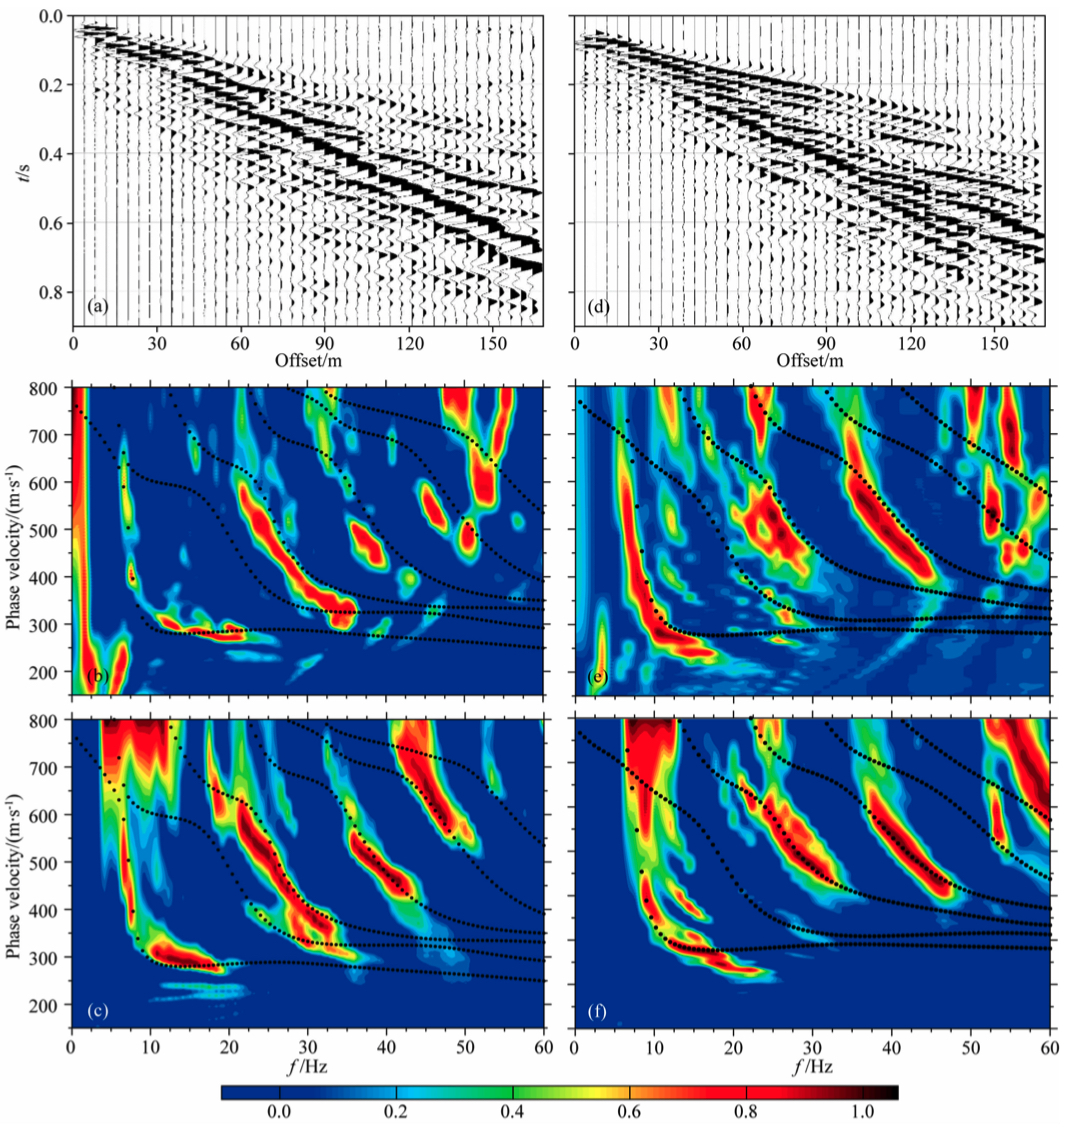
\includegraphics[width=0.85\textwidth]{imaging/fj-dispersion.jpg}
    \caption{F-J频谱能量图}
    \label{fig:fj-dispersion}
    \note{注:S25(左侧)与S35(右侧)人工炮点对应频谱图, 黑色点是预测的频散曲线点。图片引自\citep{lei2021shallow}}
\end{figure}

\begin{figure}[h]
    \centering
    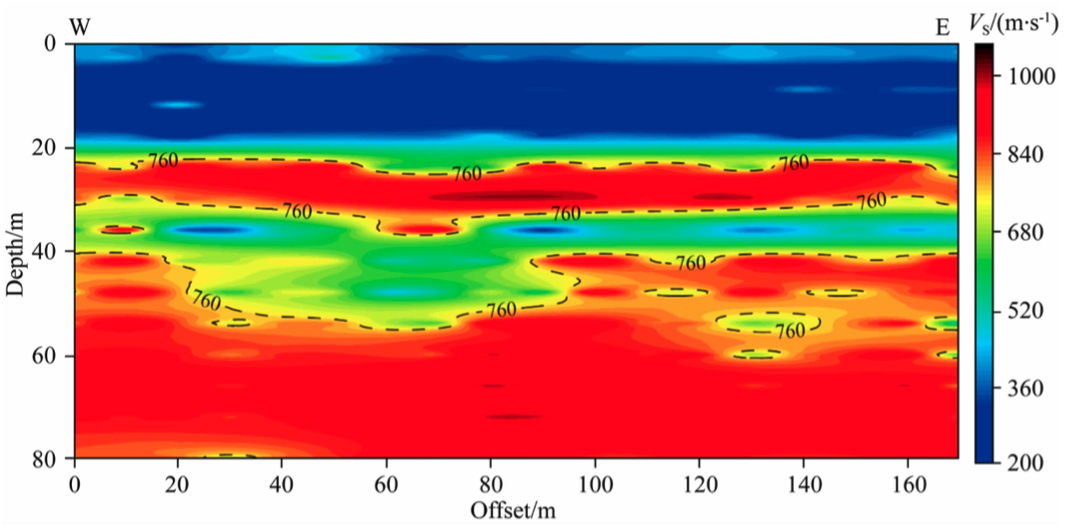
\includegraphics[width=0.85\textwidth]{imaging/2d-velocity-fj.jpg}
    \caption{高阶频散信息反演的二维速度结构}
    \label{fig:2d-velocity-fj}
    \note{注:图片引自\citep{lei2021shallow}}
\end{figure}

% 